\documentclass{article}

\usepackage{caption}
\usepackage{enumitem}
\usepackage{graphicx}
\usepackage{float}
\usepackage[section]{placeins}
\usepackage{amssymb}

\usepackage[
	backend=bibtex
]{biblatex}
\addbibresource{refs.bib}
\captionsetup{
	labelfont=bf,
	font=small,
	justification=centering
}
\renewcommand{\figurename}{Fig.}

\usepackage[
	hypertexnames=false,
	colorlinks=true,
	citecolor=blue
]{hyperref}

\title{
	Canning for Amorphous Blob Computing\\
	\small TER report
}

\author{
    Auteur~:\\
    Lucas Labouret\\
    M1 QDCS, Université Paris-Saclay\\
    \small lucas.labouret@universite-paris-saclay.fr
    \and
    Encadrant~:\\
    Frédéric Gruau\\
    LISN\\
    \small frederic.gruau@universite-paris-saclay.fr
}

\date{}

\begin{document}
 
\maketitle

\begin{figure}[H]
	\centering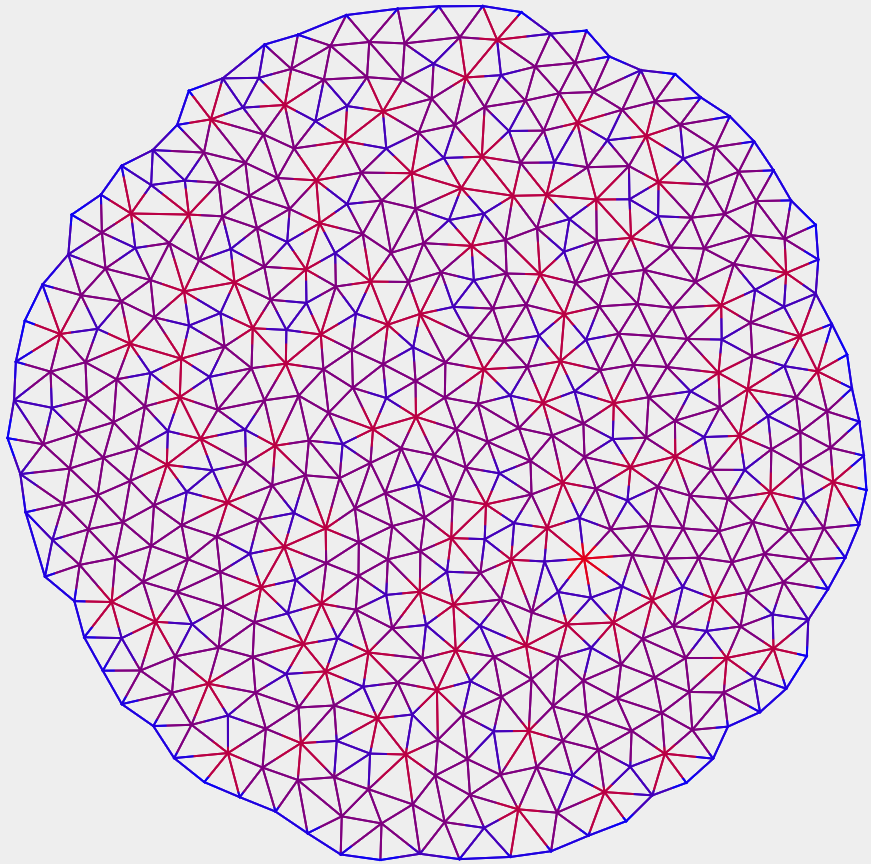
\includegraphics[width=0.9\linewidth]{assets/Circle500.png}
\end{figure}

\newpage
\tableofcontents
\newpage

\renewcommand{\thesection}{\Alph{section}}

\section*{Introduction}
\label{introduction}
\addcontentsline{toc}{section}{\nameref{introduction}}

This TER took place at the LISN from January to April 2025 under the supervision of Frédéric Gruau. It is the continuation of a research project I did under him last year as part of my Licence degree's curriculum. It is part of a long term research project about the concept of "blob computing"\supercite{blob_computing1}. During this TER, I performed research about the simulation of blob computing on classical computers, and wrote a GUI application that allows to visualize and interact with my results.

\section{What is Blob Computing ?}

To understand the exact subject of this TER, it is important to first introduce what blob computing means and how it works.\\

The ultimate goal of the project is to develop a new paradigm of computation that is inherently arbitrarily scalable through the use of \textit{space} as a resource. This kind of computation is becoming increasingly useful, for example with the recent development of swarm robotic\supercite{swarm_robotic}.

We aim to achieve this through the use of arbitrarily many processing elements (PEs) distributed through space and locally connected. These PEs, which can be severely lacking in power on their own, create a computing medium where virtual "blobs" can form and evolve. These blobs are the main primitive we use for making computations.

\subsection{Definition and Structure of a Computing Medium}

\begin{figure}[h]
	\centering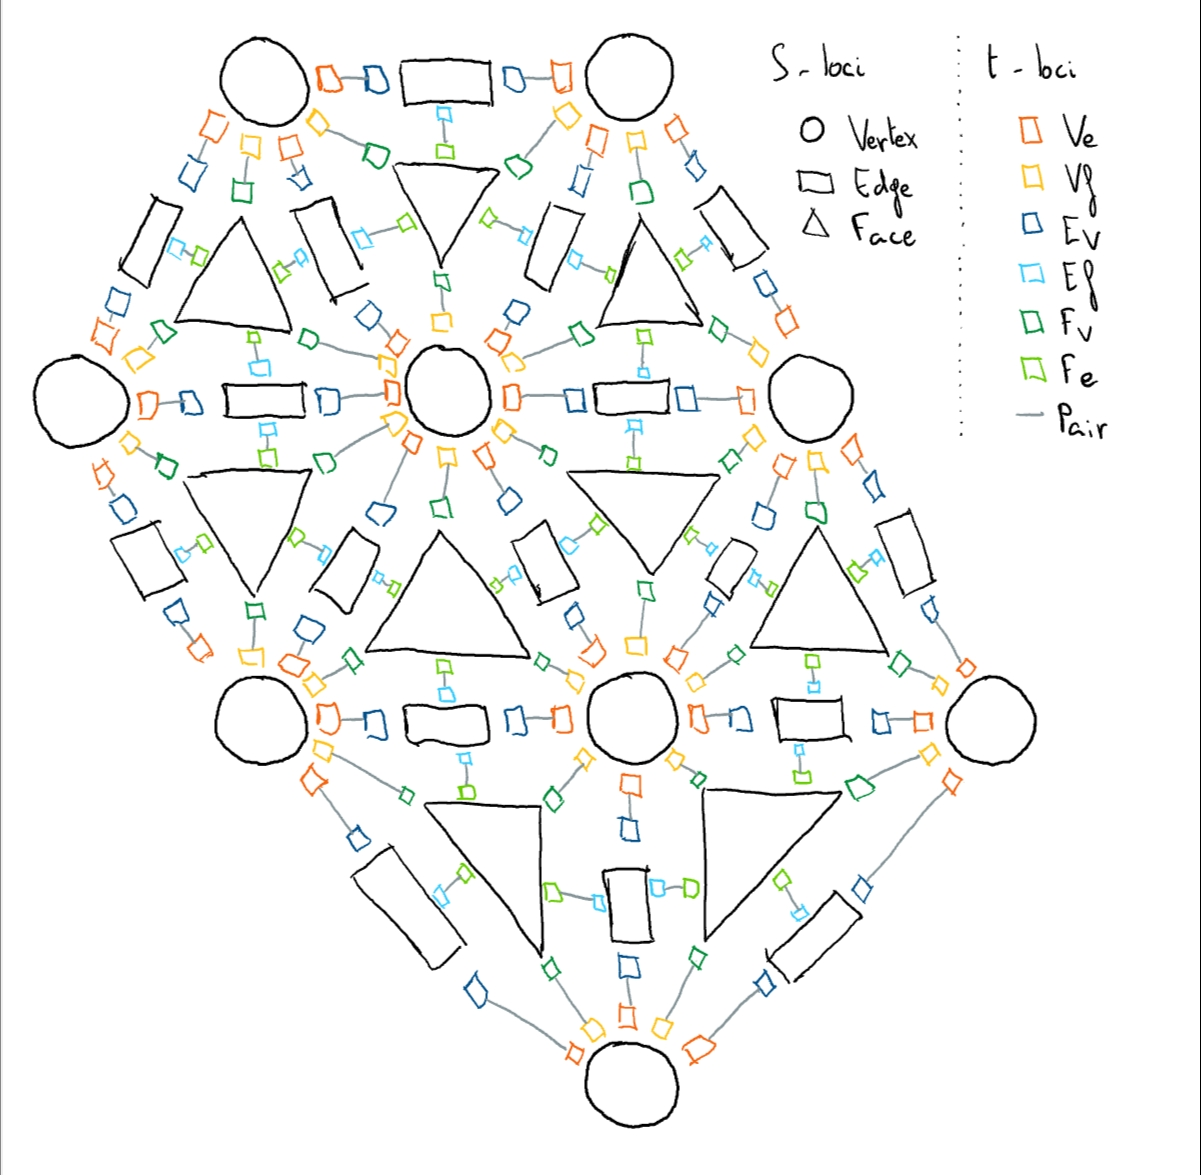
\includegraphics[width=0.9\linewidth]{assets/handdrawn_medium.png}
	\caption{Example of triangulated medium.}
	\label{fig:example_structure}
\end{figure}

In its most general form, a computing medium is simply a set of processing elements distributed in some space which are locally connected. Here, we focus exclusively on a specific kind of media called "triangulated computing media", hence the term "computing medium" in the rest of this report will refer to those unless specified otherwise. A triangulated medium is represented as a weakly Delaunay-triangulated graph where each vertex, edge, and face is associated with a processing element capable of executing minimal computation, storing information, and communicating with its neighbors.

Vertices, edges and faces are called "simplicial loci" (or "S-loci" for short). They determine the overall structure of their medium. Each S-locus controls a set of "transfer loci" (or "t-loci"). T-loci come in pairs that handle the communication between two S-loci. For example, if a vertex was connected to an edge, there would be a pair of t-loci (one belonging to the vertex and the other belonging to the edge) between them.

Obviously, there are 3 types of S-loci~: Vertex, Edge, Face. T-loci are divided into 6 types~: 
\begin{itemize}[noitemsep,nosep]
	\item Ve linking a  Vertex to an Edge
	\item Vf linking a  Vertex to a  Face
	\item Ev linking an Edge   to a  Vertex
	\item Ef linking an Edge   to a  Face
	\item Fv linking a  Face   to a  Vertex
	\item Fe linking a  Face   to an Edge
\end{itemize}
Figure~\ref{fig:example_structure} show an example of how all these loci are put together to form a medium. For reference, a vertex controls any number of Ve's and Vf's, an edge controls two Ev's and two Ef's, and a face controls three Fv's and three Fe's.

A medium is said to be crystalline if a repeating structure emerges in the placement if its vertices. It is amorphous when no such structure emerges. Additionally, it is homogeneous if the average point density is approximately constant and there are no
“holes” or “clusters”, and it is isotropic if the directions of the edges of the medium follow a uniform distribution over $[0, \pi[$. This report mainly focuses on amorphous homogeneous isotropic (AHI) media.

\begin{figure}[h]
	\centering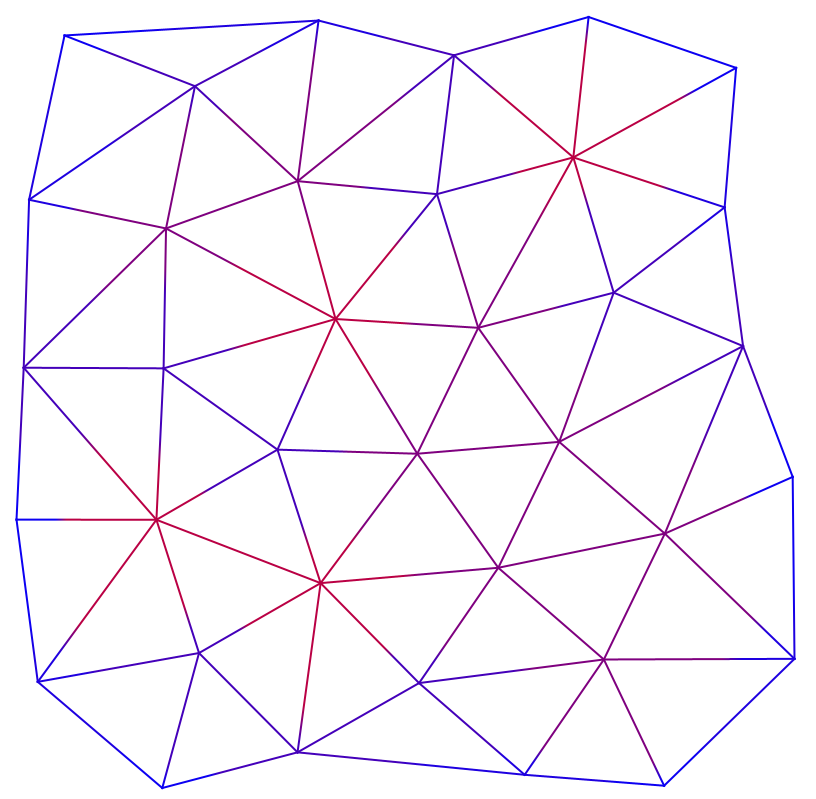
\includegraphics[width=0.4\linewidth]{assets/amorphous_medium.png}
	\hspace{0.1\linewidth}
	\centering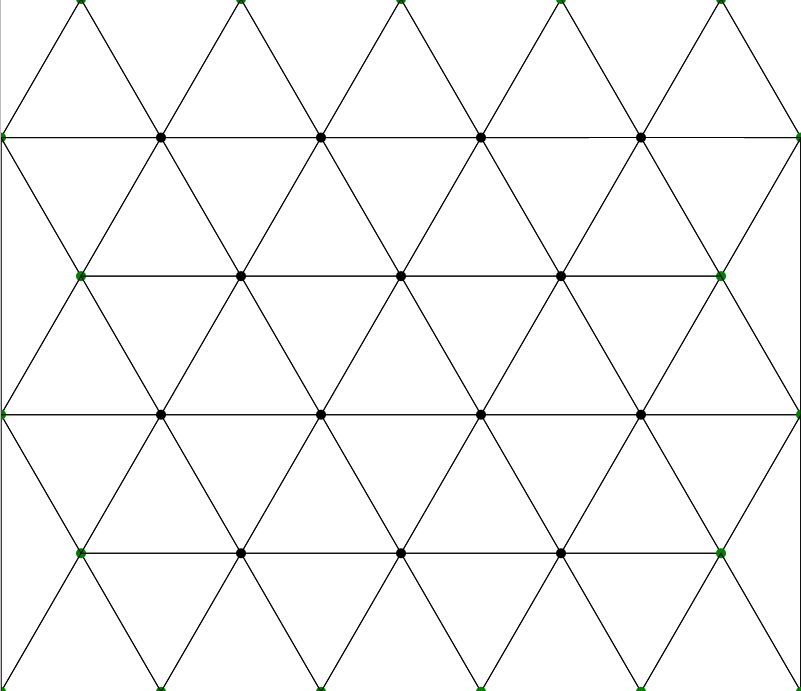
\includegraphics[width=0.4\linewidth]{assets/hexagonal_medium.png}
	\caption{An AHI medium (left) VS a crystalline hexagonal medium (right).}
	\label{fig:amorphous_vs_crystaline}
\end{figure}

For now, we consider PEs to be immobile and synchronous, although lifting these two constraints will probably be the subject of future research.\\

Blobs form the computational basis of blob computing. A blob of a given medium $M$ is a connected sub-graph $M'$ of $M$ such that all the vertices of $M'$ share a common property (e.g.: all their values are even, or all their values are 1, etc.). Formally, it is a "True" connected component of a boolean field over the vertices (see \cite{Voronoi}).

Importantly, blobs are persistent through time, meaning that two blobs at two different points in time can be considered one and the same under the right conditions, even though blobs are able to change their shape over time. This is possible for two reasons~:
\begin{enumerate}[noitemsep, nosep]
	\item Blobs maintain their connexity, they typically don't merge or divide unless instructed otherwise.
	\item Blobs only change shape at their border~: at each time step they can grow to unoccupied vertices adjacent to their border, or they can lose vertices that are part of their border.
\end{enumerate}
Therefore, two blobs at two consecutive timestep are "the same blob" if they only differ at their border. We can then extend the notion to any number of timestep through its transitive closure.

\subsection{An Example of Computation~: the Voronoï Diagram}

\cite{Voronoi} develops tools to program on computing media. As an example, it shows how to build a (discrete) Voronoï diagram from a set of "seeds" in a medium.

\begin{figure}[h]
	\centering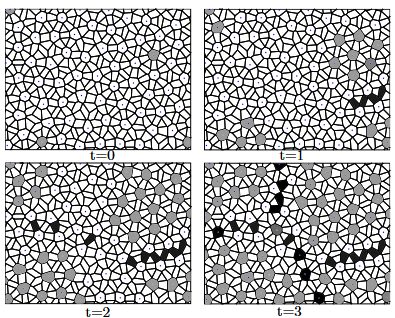
\includegraphics[width=0.7\linewidth]{assets/voronoi_spread.png}
	\caption{
		Computation of a discrete Voronoï diagram.\\
		Cells marked with a dot are the vertices of the medium.
		Gray cells form blobs. Black cells mark the frontiers between blobs. At t=0, blobs only cover the seeds. At t=3, blobs cover the Voronoï regions of the medium.\\
		\textit{Source~: \cite{Voronoi}}
	}
	\label{fig:voronoi_spread}
\end{figure}

The basic idea is the following~: we start with a set of "seeds" distributed over the vertices of the network. Each seed is now the center of a blob. Then, at each synchronous step, the blobs will spread to their adjacent vertices if this wouldn't cause them to merge with another blob, until no blob can spread further. It can be implemented with very few types of local operations that are applied simultaneously to every S-locus in the network~:
\begin{itemize}
	\item Multi-cast\\
	The S-locus copies its value into its t-loci of a given type.
	\item Rotation\\
	Since t-loci are spatially arranged around their S-loci, we can define a clockwise and counter-clockwise neighbor. T-loci can perform logical operations on their and their neighbors' values.
	\item Reduction\\
	The S-locus stores the result of a commutative and associative operation applied to the values of its t-loci of a given type.
	\item Transfer\\
	Each of the S-locus' t-loci exchanges its value with the value of its pair. 
\end{itemize}
In fact, clever association of these primitives allows to program everything a computing medium is capable of, such as sorting arrays of integer or multiplying matrices\supercite{blob_computing2}.

\subsection{Objective~: Cannings}

Up until now, Gruau mainly focused on hexagonal crystalline media. He built a plateform allowing efficient simulation of blob computation on classical hardware using SIMD\supercite{Voronoi, platform_CA2}. 

The point of this TER is to allow the use of SIMD to optimize the simulation of AHI media as well. We do this through the development of the notion of "total canning", or simply "canning". Given a medium $M$, a canning is a set of 9 injective maps which assign some integer coordinates to each locus of $M$~:
\begin{enumerate}[noitemsep,nosep]
	\item $\{$Vertex$_M\} \mapsto \mathbb{N}^{a_1}$
	\item $\{$Edge$_M\} \mapsto \mathbb{N}^{a_2}$
	\item $\{$Face$_M\} \mapsto \mathbb{N}^{a_3}$
	\item $\{$Ve$_M\} \mapsto \mathbb{N}^{a_4}$
	\item $\{$Vf$_M\} \mapsto \mathbb{N}^{a_5}$
	\item $\{$Ev$_M\} \mapsto \mathbb{N}^{a_6}$
	\item $\{$Ef$_M\} \mapsto \mathbb{N}^{a_7}$
	\item $\{$Fv$_M\} \mapsto \mathbb{N}^{a_8}$
	\item $\{$Fe$_M\} \mapsto \mathbb{N}^{a_9}$
	\item[] where $a_1, ..., a_9 \geq 1$ are specific to each canning method and designate the number of coordinates assigned to each type of locus.
\end{enumerate}
Through misuse of language, the term "canning" will designate either this set of maps, or the algorithm used to build it.

The objective is twofold~: firstly, we want to find a way to measure the efficiency of a canning on a given medium. Secondly, we want to create a canning that is efficient on most -if not all- media.

\section{Preliminary Work}

In this section, I briefly introduce some work I did last year during another internship with Gruau to generate AHI media. While it isn't the main focus of this year's TER, it is what made it possible in its current form.

\subsection{Delaunay Triangulation}

A Delaunay triangulation is a particular type of triangulation where a triplet of vertices form a face iif no other vertex can be found inside the circumcircle of the triplet. We relax this definition slightly by allowing the hull of the graph not to be convex. It presents interested properties for our purpose as the edges of the triangulation tend to remain "localized" (i.e. vertices that are connected tend to be spatially close).

I used the triangulation algorithm described in \cite{build_delaunay}. However, there is a bug in my implementation where vertically-aligned are often handled incorrectly, which I couldn't fix before the end of my internship last year. Since this problem wasn't particularly consequential this year either, I didn't take the time to fix it this year either.

Additionally, the FPO algorithm (see \ref{fpo}) performs a lot of removals and insertions to the set of vertices. Currently, each time this happens, the entire set is retriangulated. This is a vastly inefficient approach to the problem. If I had the time, I would've liked to implement the removal and addition algorithms described in \cite{build_delaunay, remove_delaunay}.

\subsection{Farthest Point Optimization}
\label{fpo}

The Farthest Point Optimization algorithm \supercite{FPO} allows the construction of the irregular yet homogeneous sets of points that we need for blob computing. It yields better results than more common algorithm like Poisson-Disk sampling or Lloyd algorithm, and fits naturally into the project as it relies heavily on the Delaunay triangulation.

The implementation of FPO in my case wasn't straightforward. This is because the article applied the algorithm to sets of points in the unit torus, while the media use bounded subsets of the Euclidean plane instead. In particular, I had to adapt the algorithm to work around the existence of borders with no predetermined shape, and that can contain fixed points that cannot be moved even though they can still influence the placement of other points.

\renewcommand{\thesection}{\arabic{section}}
\setcounter{section}{0}

\section{Borders and Media}

The border of a medium is the set composed of both the edges separating the outer face of the graph from the inner faces of the graph, and the vertices at the ends of those edges.

The method we chose to handle the borders of our media is crucial, as impacts how the media are optimized, how they are canned afterward, and decide some useful properties they have for performing computations. Ultimately, we decided to study two broad types of borders : "soft" and "hard" borders.

\subsection{Soft Borders}

Soft borders are the least restrictive of the two types. A medium has a soft border if all of its vertices are allowed to be moved anywhere in a bounded, connected region of the Euclidean plane during FPO. This region can take any shape.

This method of handling the border tends to connect vertices that would normally be too far apart from each other if they were on the inside of the medium, breaking its locality. To solve this issue, we allow the iterative removal of the edges of the border that connects points which would otherwise be "too far apart".

We initially considered two types of soft bordered media : soft square media, where the vertices are confined into a square, and soft circle media, where the vertices are confined into a circle. However, we quickly abandoned soft circle media as they currently don't have any application for computing.

\subsection{Hard Borders}

A hard bordered medium is a media whose border (both the edges and the vertices) is fixed even before FPO. Hard borders are a lot more restrictive than soft borders, but they also offer many advantages over them. In particular, since we can decide the placement of the vertices of the borders, it means they can arranged in a way that makes them easy to mirror or to fold into tori. This has interesting properties once the media is used for computation.

However, one must be careful when constructing such media, as over/under-filling can lead to a loss of homogeneity or locality near the border.

We focused on two types of hard border : a hard square with evenly placed vertices, and a hard rectangle with ratio $1\colon\sqrt{3}$. Initially, we also tried to work with a border following a hexagonal lattice to approach previous work, but we ended dropping the idea as we would either experience the loss of homogeneity/locality mentioned above, or FPO would end converging back to a hexagonal crystal, losing the isotropicism of the media.

\subsection{About Hybrid Borders}

We also briefly considered using a hybrid type of border by allowing the vertices of the borders to move in a restricted manner, we ultimately decided against it as it made our hypothesis more restrictive than pure soft borders while bringing non of the advantages that hard borders have.

\section{Canning and Evaluation}

Before we begin our search for total cannings, let us define the notion of partial canning. A partial canning of a medium $M$ is simply a subset of a total canning of $M$ (or the algorithm used to build it). In particular, we focus on vertex cannings, i.e. partial cannings which only contain the map from the vertices of $M$ to their coordinates. From there, we will exhibit a generic method for build total cannings using vertex canning as a base. Finally, we will show how we can evaluate the efficiency of different cannings so we can compare them.

\subsection{Vertex Cannings}
\label{partial_canning}

To align with the way crystaline media are hendled, we set $a_1 = 2$, i.e. we want to assign 2D integer coordinates to each vertex of the medium. The problem now becomes equivalent to placing the vertices in a 2D grid. The vertex canning is valid if all the vertices have been placed in the grid and if each cell of the grid contains at most one vertex. The coordinates of each vertex then becomes the 2D index of its cell. Based on this idea, I have developped two diffrent vertex cannings with opposite philosophies~:
\begin{enumerate}
	\item \textbf{TopDistanceXStorted} vertex canning\\
	This vertex canning was developed to rely as much as possible on the graph structure of the medium, making as little use as possible of its embedding. It was developed quite early in the project, before soft-bordered media appeared, so it only works on hard-bordered media. It works in the following way~:\\
	- First, compute the minimum graph-distance of each vertex to any vertex on the topside of the border. All vertices at distance Y from the top are placed in line Y of the grid.\\
	- Second, place the leftmost vertex of each line in the first cell of its line, the second leftmost vertex of each line in the second cell of its line, repeating until all vertices are placed in the grid.
	
	\item \textbf{RoundedCoordinates} vertex canning\\
	This vertex canning was developed to rely exclusively on the spatial embedding of the medium, completing ignoring its graph structure. It works in the following way~:\\
	- First set a counter to 1.\\
	- Multiply the spatial coordinates of each vertex by the counter and round the result. Use the two integers obtained as a 2D index to put each vertex in the grid.\\
	- If two vertices share the same cell, increment the counter by one and go back to the previous step. Otherwise, we have a vertex canning.
\end{enumerate}

Regarding the TopDistanceXStorted algorithm, I first tried sorting the lines using the distance to the leftside border, however it resulted in invalid vertex cannings where two vertices would share the same cell.

\begin{figure}[h]
	\centering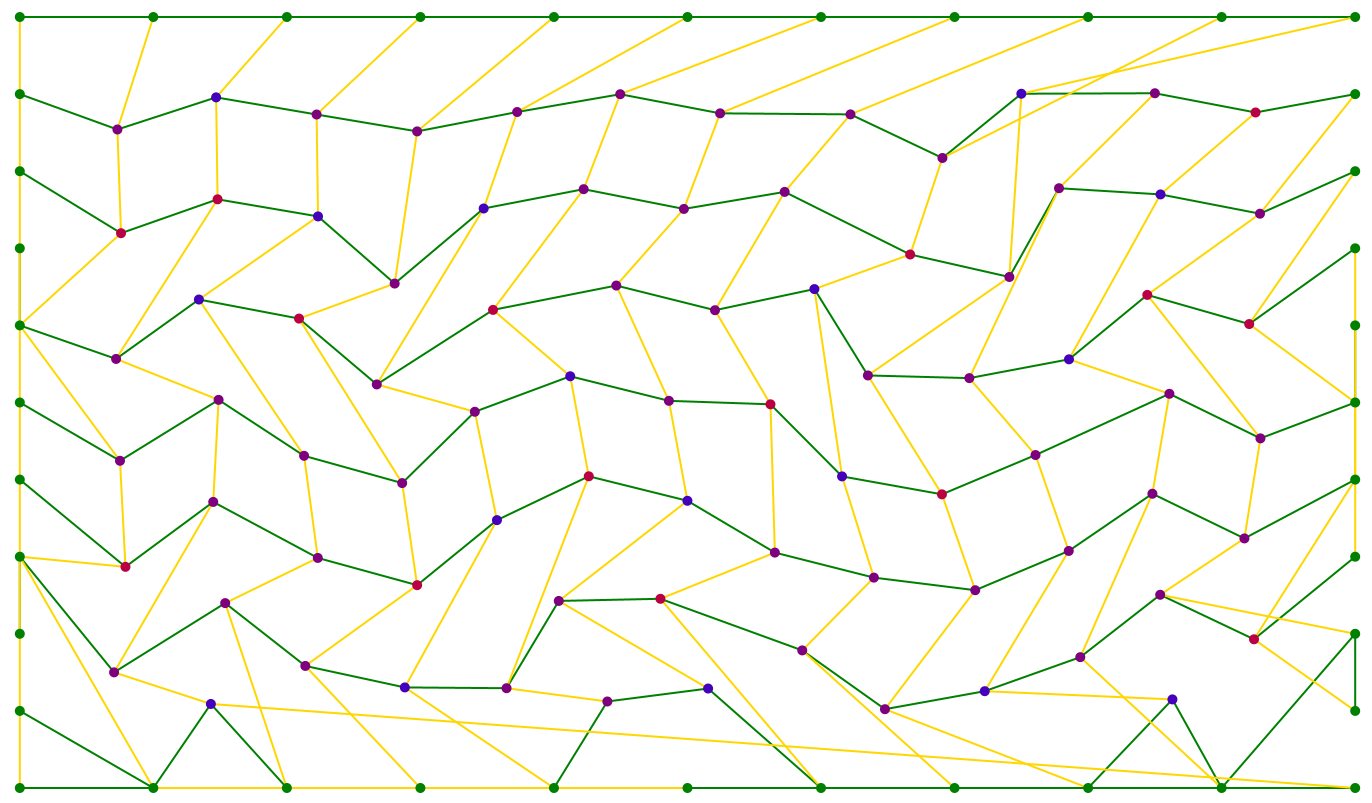
\includegraphics[width=0.45\linewidth]{assets/TopDistanceXSorted.png}
	\centering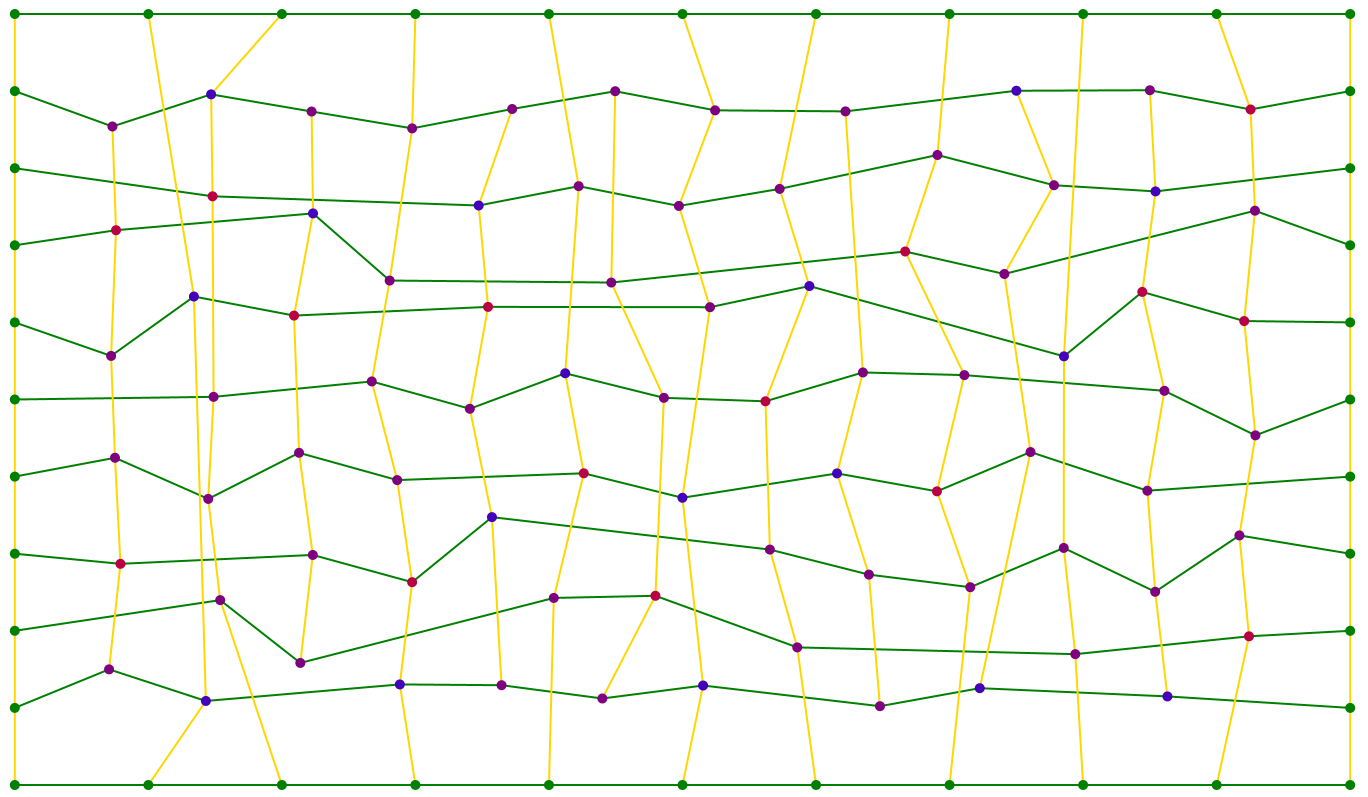
\includegraphics[width=0.45\linewidth]{assets/RoundedCoordinates.png}
	\caption{TopDistanceXSorted (left) next to RoundedCoordinates (right) applied to the same medium.\\
	Two vertices are joint by a green line if they are consecutive on a line of the grid, and a yellow line if they are consecutive in a column.}
	\label{fig:topdist_vs_rounded}
\end{figure}

Intuitively from figure~\ref{fig:topdist_vs_rounded}, we can infer that RoundedCoordinates is better as it creates a more "grid-like" canning, whereas the columns in TopDistanceXSorted seem to "drift" to the left. We will confirm this intuition later.

\subsection{From Vertex to Total Cannings}

Now that we can build vertex cannings, we want a method to convert them into total cannings.

To do this, we first define the "belonging" relation between loci, such that we can say that some locus A belongs to some other locus B. We do this so that can "index" B relative to A. Given some vertex canning $VC$, we define the relation in the following way~:
\begin{itemize}
	\item Vertices belong to no one.
	\item We iterate over the lines of $VC$, going from the top-most line to the bottom-most line in order.\\
	Then we iterate over each vertex $V$ of the line, going from the left-most to the right-most in order.\\
	Each Edge and Face connected to $V$ now belong to $V$, unless it already belongs to another vertex.
	\item Each t-locus belongs to the S-locus that has control over it.
\end{itemize}
Now, given a vertex $v$, an edge $e$ and a face $f$ we write
\begin{itemize}[noitemsep, nosep, label=-]
	\item $y_v$ and $x_v$ the coordinates of $v$ in $VC$,
	\item $E(v)$ the set of edges belonging to $v$,
	\item $F(v)$ the set of faces belonging to $v$,
	\item $Ve(v)$ the set of Ve t-loci belonging to $v$
	\item $Vf(v)$ the set of Vf t-loci belonging to $v$
	\item $Ev(e)$ the set of Ev t-loci belonging to $e$
	\item $Ef(e)$ the set of Ef t-loci belonging to $e$
	\item $Fv(f)$ the set of Fv t-loci belonging to $f$
	\item $Fe(f)$ the set of Fe t-loci belonging to $f$\\
\end{itemize}

Since the edges, faces, Ve's and Vf's will be indexed relative to vertices, we set $a_2 = a_3 = a_4 = a_5 = a_1+1 = 3$. Similarly, Ev's and Ef's will be indexed relative to edges so we set $a_6 = a_7 = a_2+1 = 4$, and Fv's and Fe's will be indexed relative to faces so we set $a_8 = a_9 = a_3+1 = 4$. Now, the attribution of coordinates works in the following way :
\begin{itemize}
	\item \textbf{Edges}~:\\
	For each vertex $v$
	\begin{itemize}[noitemsep, nosep, label=-]
		\item Select a first edge. If it exists and it is in $E(v)$, it is the edge joining $v$ to the next vertex in its line. Otherwise, start on the left of $v$ and walk clockwise around it, selecting the first edge in $E(v)$ that you cross.
		\item Sort $E(v)$ clockwise around $v$ starting from your first edge.
		\item Number your edges, starting at 0 and incrementing by 1 in the order of your sorted $E(v)$.
		\item Edge number $p$ now has coordinates $(p, y_v, x_v)$.
	\end{itemize}
	
	\item \textbf{Faces}~:\\
	For each vertex $v$
	\begin{itemize}[noitemsep, nosep, label=-]
		\item Select a first face. If it exists and it is in $F(v)$, it is the face joining $v$ to the next vertex in its line and to $v$'s next neighbor clockwise. Otherwise, start on the left of $v$ and walk clockwise around it, selecting the first face in $F(v)$ that you cross.
		\item Sort $F(v)$ clockwise around $v$ starting from your first face.
		\item Number your faces, starting at 0 and incrementing by 1 in the order of your sorted $F(v)$.
		\item Face number $p$ now has coordinates $(p, y_v, x_v)$.
	\end{itemize}
	
	\item \textbf{Ve's}~:\\
	For each vertex $v$
	\begin{itemize}[noitemsep, nosep, label=-]
		\item Select a first Ve. If it exists, it is the Ve linking $v$ to the edge joining $v$ to the next vertex in its line. Otherwise, start on the left of $v$ and walk clockwise around it, selecting the Ve in $Ve(v)$ linking $v$ to the first edge in $E(v)$ that you cross.
		\item Sort $Ve(v)$ clockwise around $v$ starting from your first Ve.
		\item Number your Ve's, starting at 0 and incrementing by 1 in the order of your sorted $Ve(v)$.
		\item Ve number $p$ now has coordinates $(p, y_v, x_v)$.
	\end{itemize}
	
	\item \textbf{Vf's}~:\\
	For each vertex $v$
	\begin{itemize}[noitemsep, nosep, label=-]
		\item Select a first Vf. If it exists, it is the Vf linking $v$ to the face joining $v$ to the next vertex in its line and to $v$'s next neighbor clockwise. Otherwise, start on the left of $v$ and walk clockwise around it, selecting the Vf in $Vf(v)$ linking $v$ to the first face in $F(v)$ that you cross.
		\item Sort $Ve(v)$ clockwise around $v$ starting from your first Ve.
		\item Number your Vf's, starting at 0 and incrementing by 1 in the order of your sorted $Vf(v)$.
		\item Vf number $p$ now has coordinates $(p, y_v, x_v)$.
	\end{itemize}
	
	\item \textbf{Ev's}~:\\
	For each Edge $e$ 
	\begin{itemize}[noitemsep, nosep, label=-]
		\item We note $(p, y_e, x_e)$ its coordinates.
		\item The Ev linking to the vertex $e$ belongs to has coordinates $(0, p, y_e, x_e)$.
		\item The other Ev has coordinates $(1, p, y_e, x_e)$.
	\end{itemize}
	
	\item \textbf{Ef's}~:\\
	For each Edge $e$ 
	\begin{itemize}[noitemsep, nosep, label=-]
		\item We note $(p, y_e, x_e)$ its coordinates, and $v$ the vertex it belongs to.
		\item We consider that $e$ "faces" $v$, which let us distinguish between a right Ef and a left Ef.
		\item The right Ef has coordinates $(0, p, y_e, x_e)$.
		\item The left Ef has coordinates $(1, p, y_e, x_e)$.
	\end{itemize}
	
	\item \textbf{Fv's}~:\\
	For each face $f$ 
	\begin{itemize}[noitemsep, nosep, label=-]
		\item We note $(p, y_f, x_f)$ its coordinates, and $v$ the vertex it belongs to.
		\item We call "first Fv" the Fv linking to $v$
		\item Starting from the first Fv, we number the Fv's 0 through 2 clockwise around $f$.
		\item Fv number $q$ now has coordinates $(q, p, y_f, x_f)$
	\end{itemize}
	
	\item \textbf{Fe's}~:\\
	For each face $f$ 
	\begin{itemize}[noitemsep, nosep, label=-]
		\item We note $(p, y_f, x_f)$ its coordinates, and $v$ the vertex it belongs to.
		\item We call "first Fe" the Fe clockwise-next to the Fv linking to $v$
		\item Starting from the first Fe, we number the Fe's 0 through 2 clockwise around $f$.
		\item Fe number $q$ now has coordinates $(q, p, y_f, x_f)$
	\end{itemize}
\end{itemize}

\subsection{Evaluation}

\subsubsection{Definition}

\newcommand{\footnoteConstantFactor}{
	For example, there is exactly 2 Ev per edge, and there are at most 3 times as many edges as there are vertices, so Ev-Ve communication will have a constant factor of 6.
}

Finally, now that we have total cannings, we want a way to evaluate them. First we remember that the point of a canning is to allow the use of SIMD to simulate the execution of a computing media. Therefore, we want can decide how good a canning is by deciding how many operations are needed to simulate each an execution step, and how well they can be parallelized. While it is possible to compute this exactly, for now we only focus on finding an upper bound. We do this by noticing that since
\begin{enumerate}[noitemsep, nosep]
	\item each t-locus in a canning is indexed relative to vertex and
	\item all communications are uniquely determined by the triangulated graph, which is itself (with probability 1 in general) uniquely determined by the placement of the vertices,
\end{enumerate}
we can find an upper bound for each communication type with a single computation over the canning of the vertices, which will be accurate up to a constant factor that depends on the type of communication\footnote{\footnoteConstantFactor}.

This upper is given by a $\Delta y$, which designates the maximum distance between two lines of vertices that interact with each other, and a $\Delta x$, which designates the maximum distance between two columns of vertices that interact with each other. Together, they allow computing $\mathcal{A}_{max} = (2\Delta y + 1)(2\Delta x + 1)$ the maximum area of interaction around any vertices.

Together with the constant factor we defined earlier, this $\mathcal{A}_{max}$ forms the upper bound were looking for. Therefore $\mathcal{A}_{max}$ is a suitable measurement of the performance of a canning, which we wish to minimize.

\subsubsection{Some results}

Overall, as we guessed earlier, the RoundedCoordinates algorithm yields much better results than the TopDistanceXSorted algorithm. RoundedCoordinates produces an $\mathcal{A}_{max}$ oscillating between 25 and 49 regardless of the size the medium. Meanwhile TopDistanceXSorted produces an $\mathcal{A}_{max}$ that grows with the size of the medium. It outperforms RoundedCoordinates for very small media (less than 50 vertices) but quickly becomes much worse with an $\mathcal{A}_{max}$ reaching upward of 150 for 1000 vertices, and upward of 200 for 2000 vertices.

RoundedCoordinates seems to perform overall better on (reasonably defined) hard bordered media. This aligns with our observation that soft borders join vertices that would normally be too far apart from each other, perhaps indicating that we are too lenient when initially correcting the border.

TopDistanceXSorted seems to get worse the wider the media get. This is further evidence that the "drift" in the columns we observed earlier is responsible for the poor performance of this method.

\section{GUI}

A large portion of the TER was focused on the development of a software equipped with a GUI that allows the user to
\begin{enumerate}[noitemsep,nosep]
	\item Randomly generate new media, save them, and load them.
	\item Optimize media with different parameters.
	\item Visualize different aspects of media.
	\item Compute and visualize different cannings.
\end{enumerate}
$ $

If developing a GUI for this application ended up being time-consuming, it was incredibly helpful all around while debugging everything else. Overall it was probably a net positive on development time alone, and that is still neglecting the advantage of being able to see what I am doing.\\
$ $

Below are some pictures of the kind of visualization the GUI provides.

\begin{figure}[h]
	\centering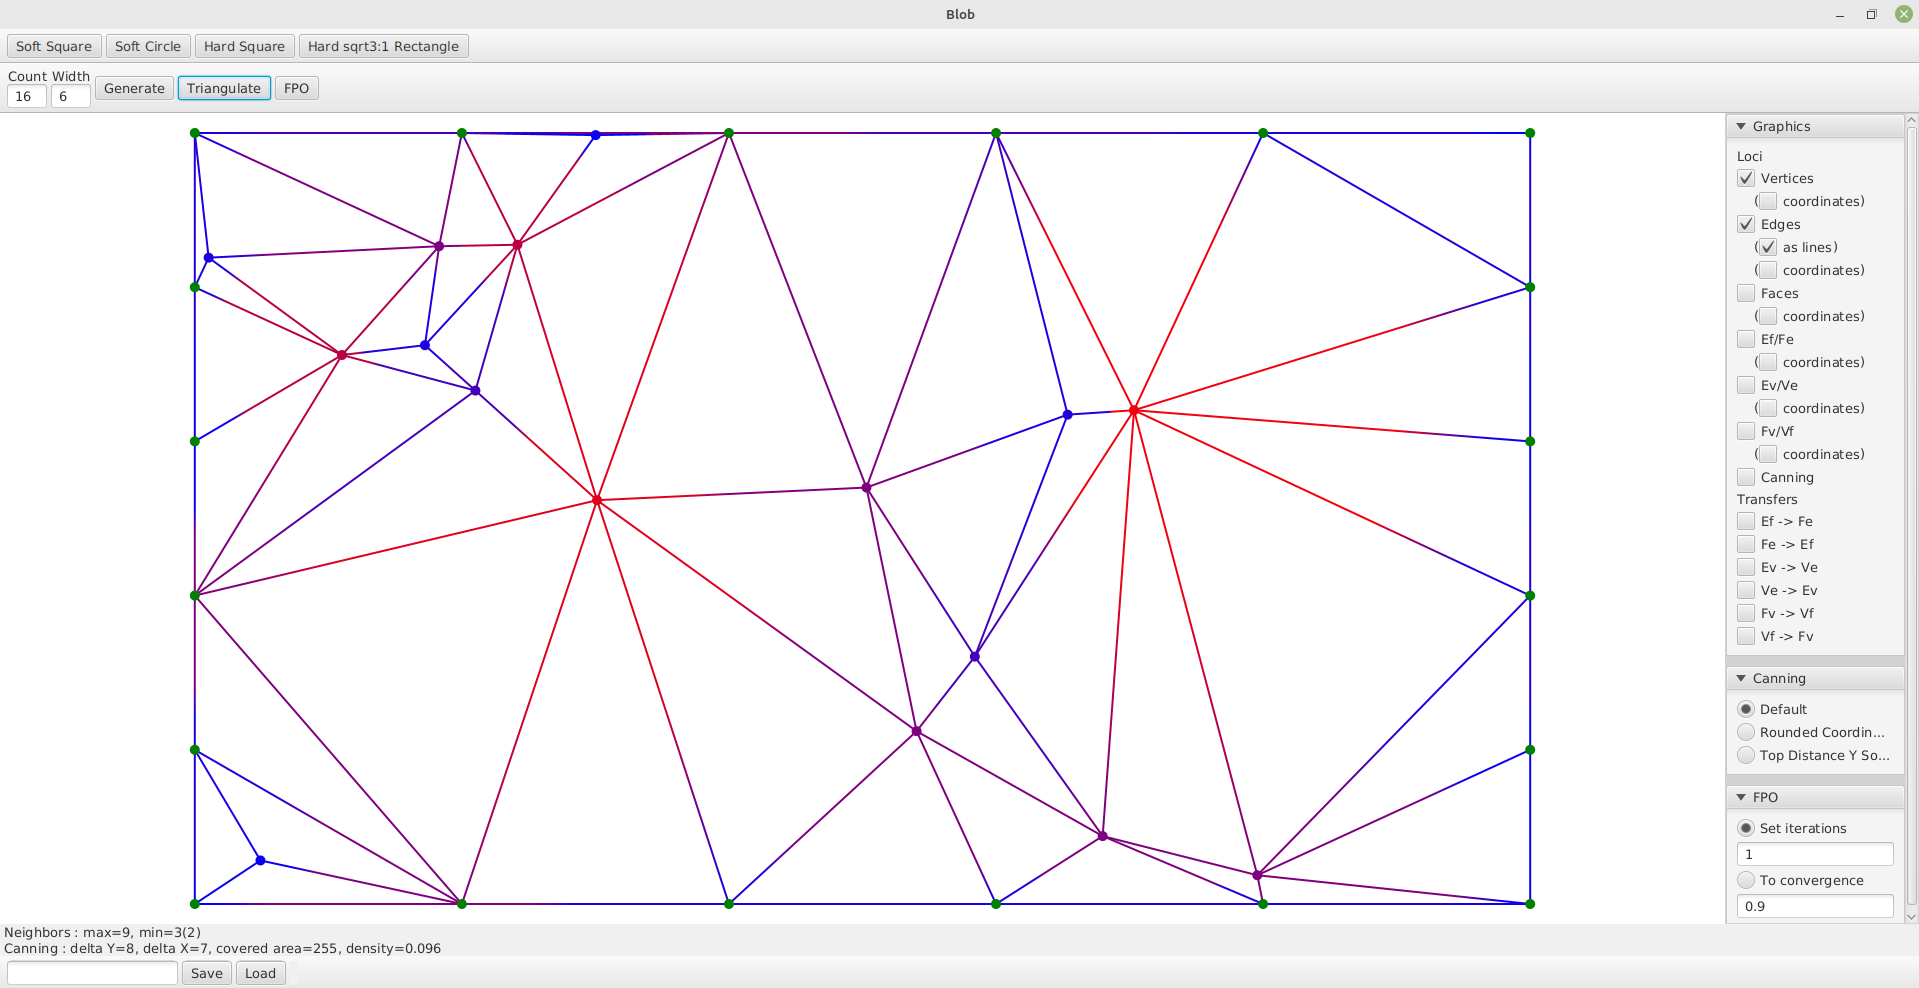
\includegraphics[width=0.45\linewidth]{assets/canonical_before.png}
	\centering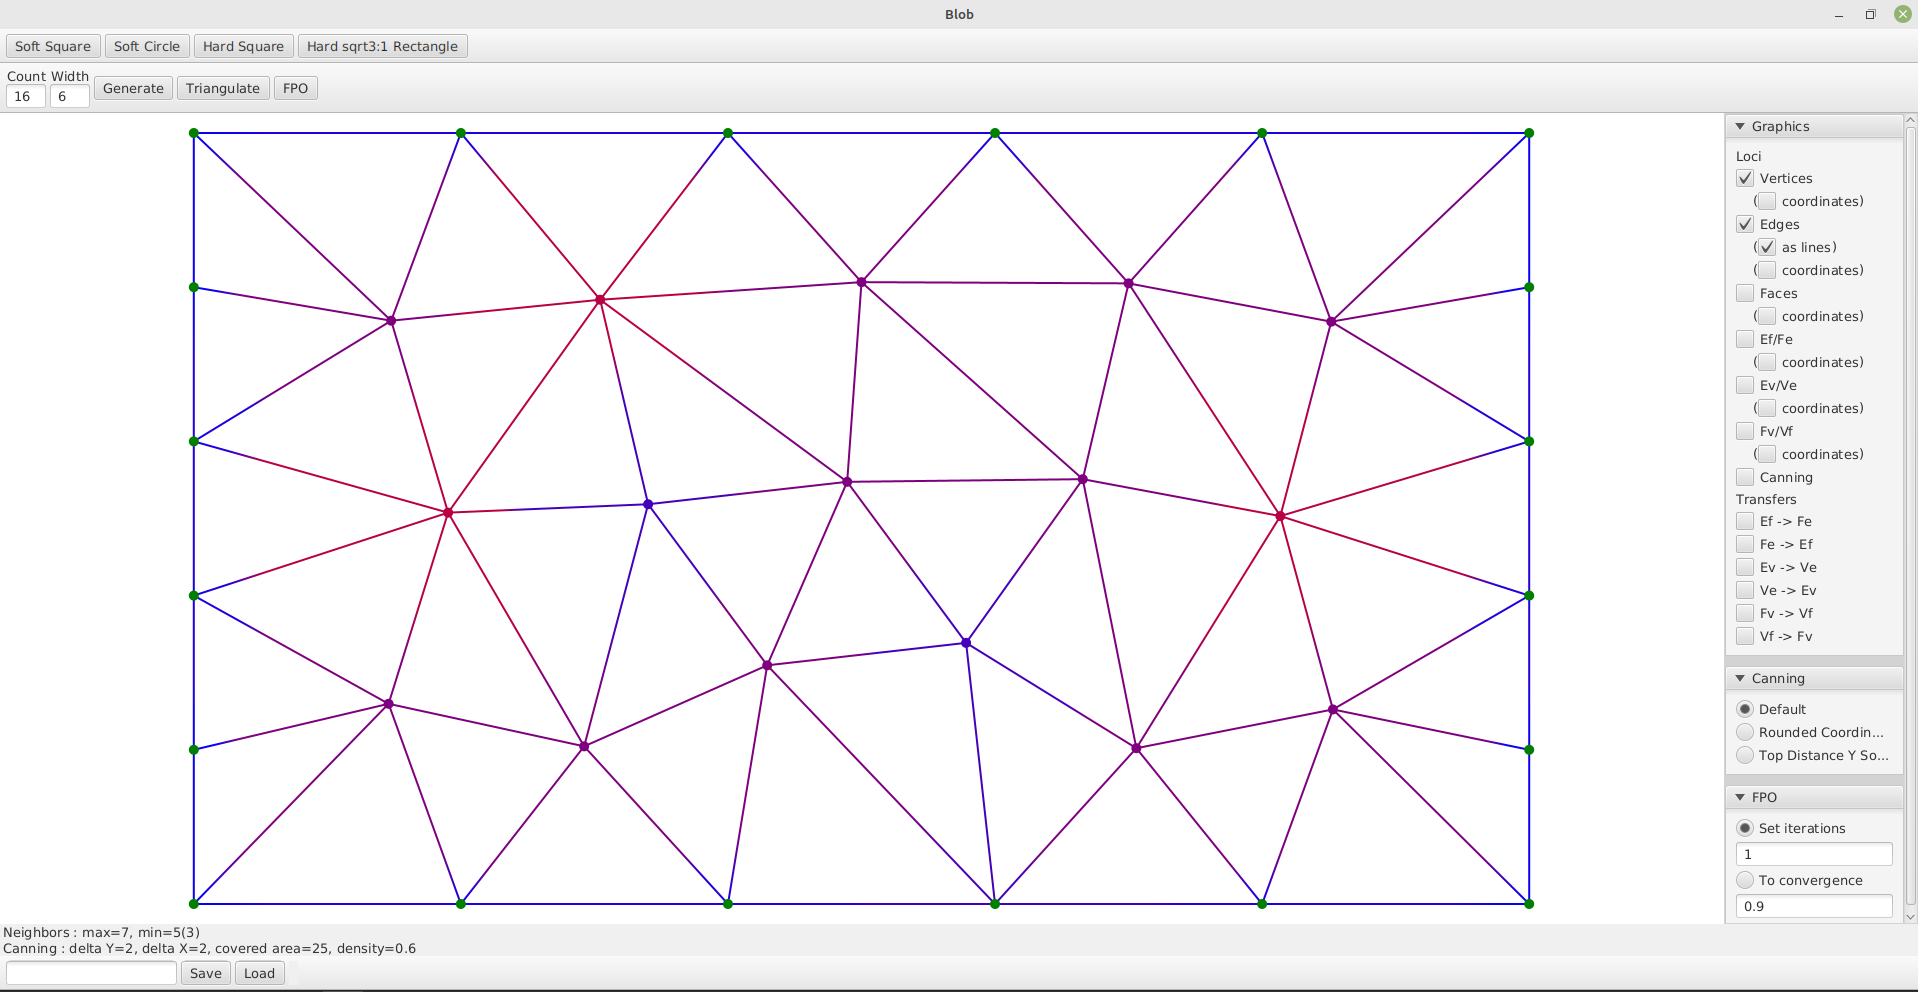
\includegraphics[width=0.45\linewidth]{assets/canonical_after.png}
	\caption{"Canonical" view of a medium before (left) and after (right) optimization with FPO.}
	\label{fig:gui_before_after_FPO}
\end{figure}

\begin{figure}[h]
	\centering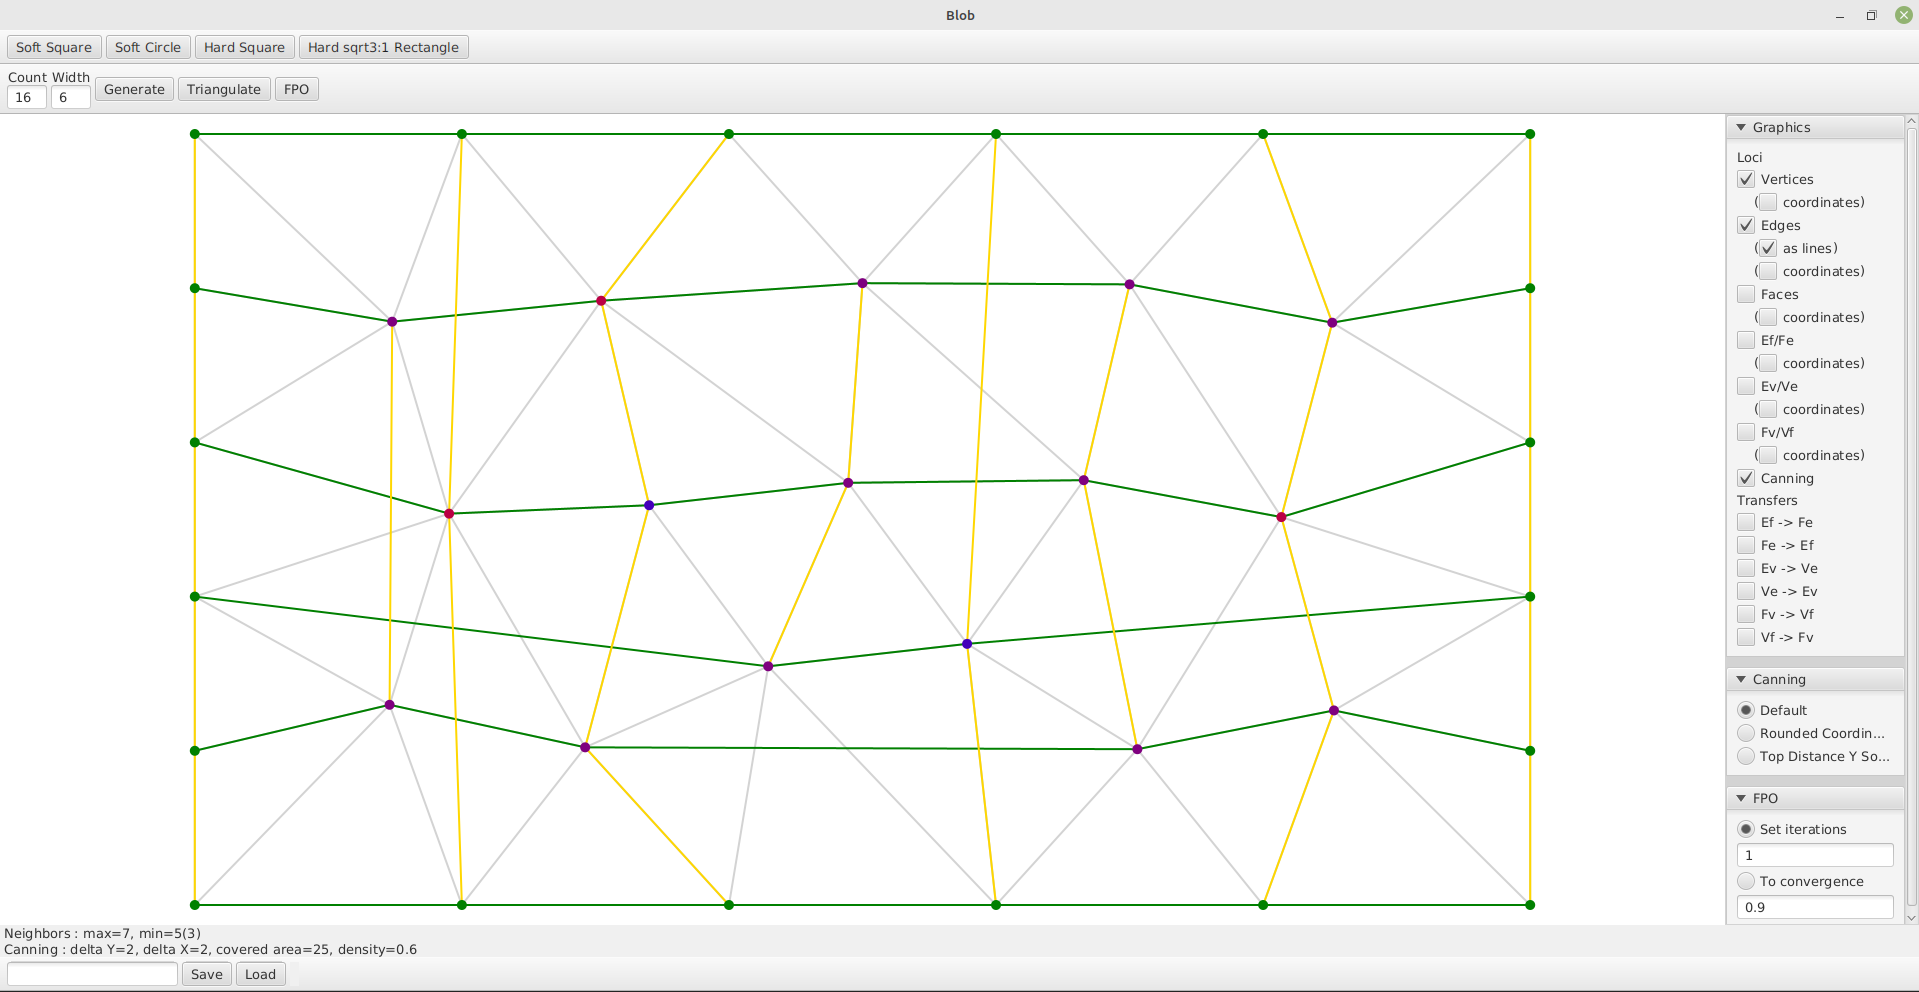
\includegraphics[width=0.8\linewidth]{assets/canning_view.png}
	\caption{View of a partial canning (see \ref{partial_canning}) of the vertices of the medium in figure~\ref{fig:gui_before_after_FPO}}
	\label{fig:gui_canning}
\end{figure}

\begin{figure}[h]
	\centering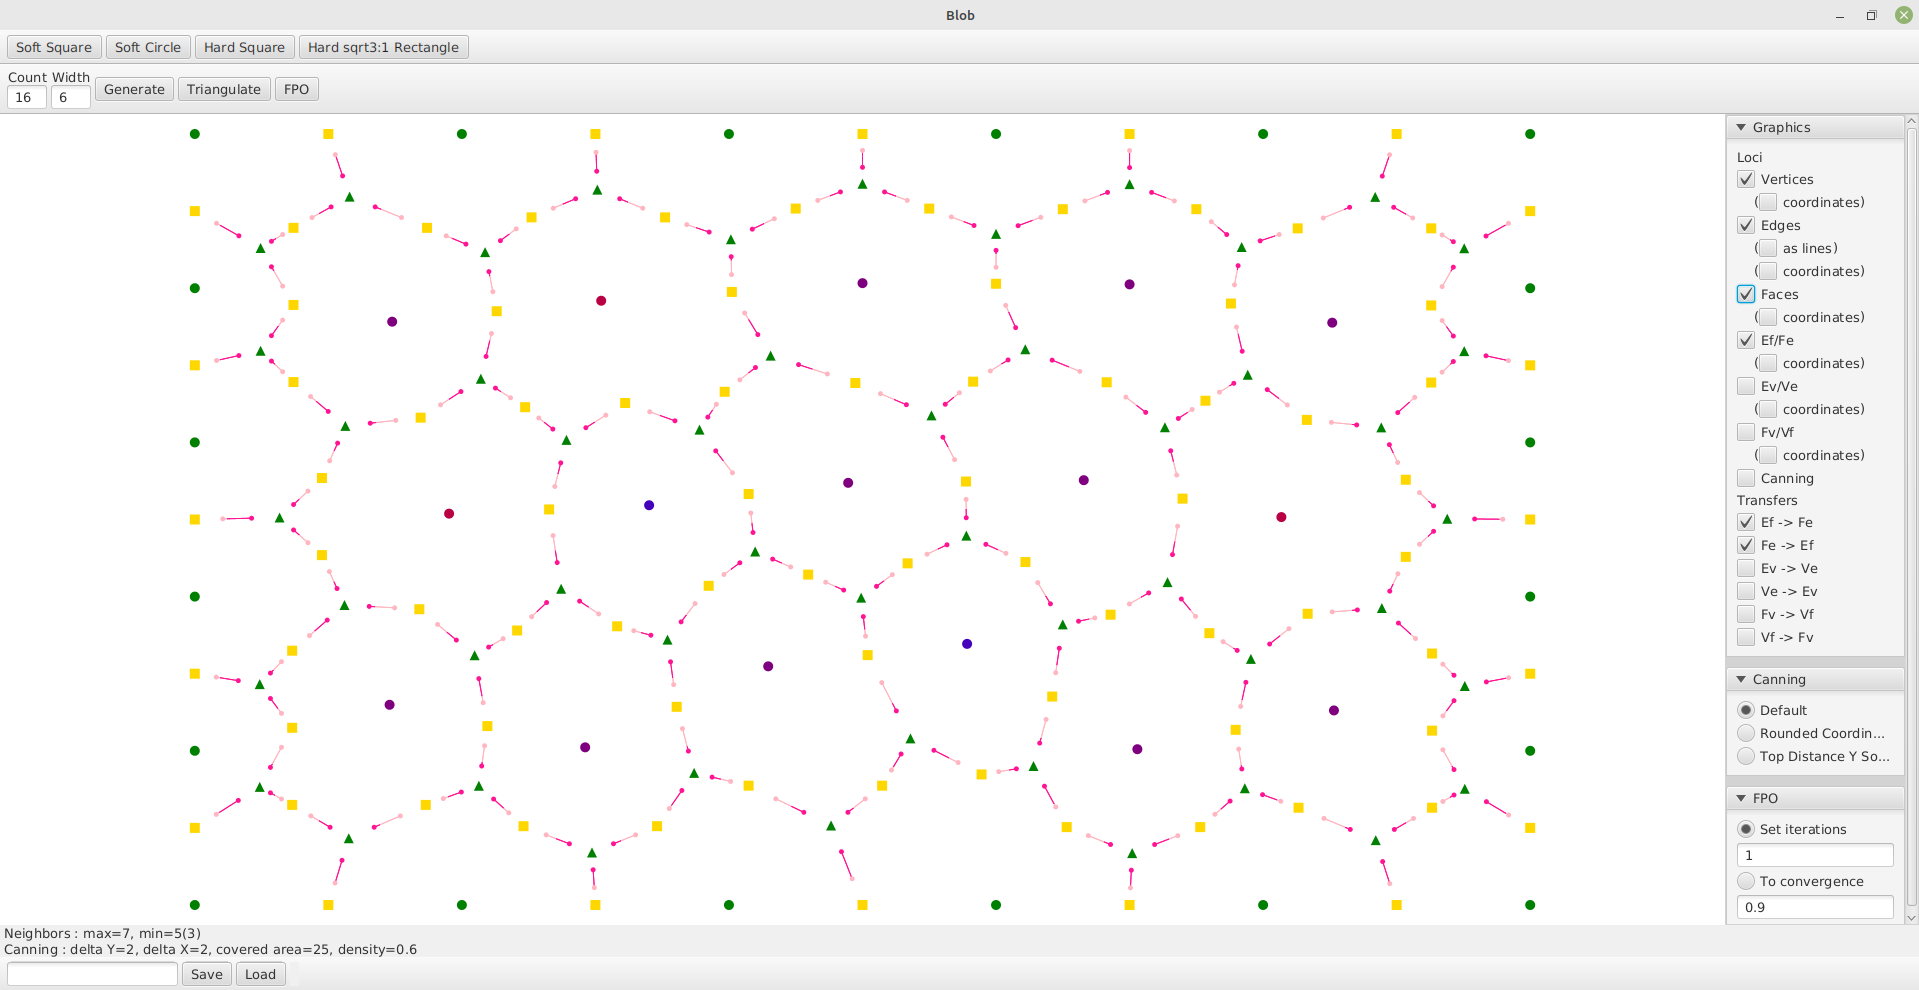
\includegraphics[width=0.8\linewidth]{assets/EfFe_transfers.png}
	\caption{View of the Ef-Fe pairs in the medium of figure~\ref{fig:gui_before_after_FPO}.}
	\label{fig:gui_EfFe}
\end{figure}

\section*{Conclusion}
\label{conclusion}
\addcontentsline{toc}{section}{\nameref{conclusion}}

\printbibliography[heading=bibintoc]

\end{document}
